\chapter{Transfer Learning}

\section{Introduction}
During the course we saw some problem that can affect the NNs like the \textbf{Overfitting}, that is when the performance on the training test are very high and on the test set very low, and the \textbf{Epistemic of Uncertainty} that essentially is the uncertainty on the learned model parameter caused by the lack of knowledge of the data.

The first idea that can be arise to solve this problems is use something like some \textbf{regularization techniques} or "simply" \textbf{collect more data}.

Another idea can be to inject \textbf{prior knowledge} into our model, in order to guide the
learning process toward more plausible solutions.  
The idea is to \textbf{reduce epistemic uncertainty by injecting prior knowledge into our model}.
This approach is known as \textbf{inductive bias}.

\subsection{Inductive Bias}
The \textbf{inductive bias} refers to the set of assumptions, constraints, or prior knowledge
encoded in a learning algorithm, which guide it to favor certain hypotheses over others.
When multiple explanations fit the training data equally well, the inductive bias determines
which hypothesis is preferred by the model.

Formally, the inductive bias $B$ of a learning algorithm $A$ can be defined as the set of
assumptions used to select a single hypothesis $h^*$ from all hypotheses consistent with the
training data. Let $H$ be the hypothesis space, $D$ the dataset, and $L$ a loss function:
\[
h^* = \arg\min_{h \in H} L(h, D) \quad \text{s.t. } h \in B
\]
where $B$ can be interpreted in two equivalent ways:
\begin{compactitemize}
    \item $B \subset H$: restriction of the hypothesis space (\textbf{restriction bias});
    \item $B : H \rightarrow \mathbb{R}$: preference ordering over hypotheses (\textbf{preference bias}).
\end{compactitemize}

Equivalently, an inductive bias can be seen as either a restriction on the set of admissible
hypotheses or as a preference among them.

Typical examples of inductive bias in modern neural architectures include:
\begin{compactitemize}
    \item \textbf{Convolutional Neural Networks (CNNs)}: assume that images exhibit locality
    and translation-invariant patterns, drastically reducing the hypothesis space;
    \item \textbf{Sparse Autoencoders}: enforce sparse representations, encouraging the model
    to capture meaningful and disentangled semantic features;
    \item \textbf{Graph Neural Networks (GNNs)}: exploit the adjacency matrix to encode structural
    priors about relationships and interactions in the domain.
\end{compactitemize}

\begin{infobox}[Note]
    Note that \textbf{Transformers} retain relatively weak inductive biases compared to CNNs or GNNs, delegating most structural assumptions to the data itself.
\end{infobox}

\subsection{Transfer Learning}
\textbf{Transfer Learning} is a learning paradigm in which knowledge acquired from a
\emph{source task/domain}, typically data-rich, is reused to improve performance on a related
\emph{target task/domain}, usually characterized by limited data availability.
This knowledge is encoded in the representations and parameters learned by the model during
pretraining.

More formally, transfer learning leverages representations learned on a source domain to bias
the learning process on the target domain.
For this reason, transfer learning can be interpreted as a particular and powerful form of
\textbf{inductive bias}.

The key assumption underlying transfer learning is that the optimal hypothesis for the target
task is likely to be similar to a good hypothesis for the source task.
Equivalently, pretraining on a source domain provides model parameters $\theta_S$ that are close
to an optimal solution $\theta_T^*$ for the target task.
As a consequence, the pretrained model acts as a strong prior, significantly reducing
\textbf{epistemic uncertainty} in data-scarce scenarios.

\subsection{Fine-Tuning}
\textbf{Fine-tuning} is the most common strategy used in transfer learning.
The idea is to first train a model on a large-scale source task and then reuse the learned
weights as initialization for training on the target task.

The typical fine-tuning procedure consists of the following steps:
\begin{compactitemize}
    \item pretrain a model (e.g. a CNN or a Transformer) on a source task;
    \item obtain the learned parameters from the source model;
    \item initialize the target model with these parameters;
    \item further train the model on the target task using the available data.
\end{compactitemize}

\begin{wrapfigure}{r}{0.3\textwidth}
    \centering
    \vspace{-10pt}
    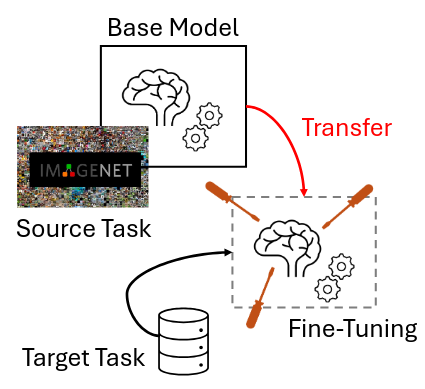
\includegraphics[width=\linewidth]{images/LT1.png}
    \label{fig:Scaled Dot Product Attention}
    \vspace{-10pt}
\end{wrapfigure}

In computer vision, a common example is pretraining a CNN on ImageNet and then fine-tuning it
for a specific task such as medical image classification.
In natural language processing, language models are often pretrained on large text corpora
(e.g. Wikipedia) and fine-tuned for downstream tasks such as sentiment analysis.

By starting from pretrained weights instead of random initialization, fine-tuning encourages
the model to exploit features that capture general and transferable patterns
(e.g. edges, textures, shapes, or semantic structures), improving generalization and reducing
the amount of data required for effective learning.

\section{Fine-Tuning}
We have seen that today the typical way to train a NN is using a fine-tuning approach, this beacuse lead to many advantage. This advantage including:
\begin{compactitemize}
    \item \textbf{Performance}: fine tuning often \textbf{outperforms} training from scratch, especially in data-scarce scenarios.
    \item \textbf{Computational constraints}: few companies can afford to train very large models from scratch.
    \item \textbf{Data availability}: large-scale dataset required for training from scratch are not always accessible.
\end{compactitemize}

\subsection{The effectiveness of Fine-Tuning}
\begin{figure}[H]
    \centering
    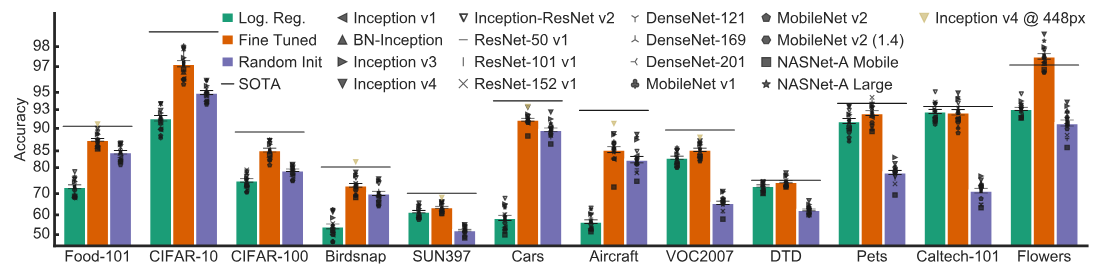
\includegraphics[width=0.9\textwidth]{images/LT2.png}
    \caption{Image from "Do better ImageNet model transfer better"}
    \label{fig:MHA2}
\end{figure}
The figure illustrates the effectiveness of \textbf{fine-tuning} compared to other strategies
for reusing or training vision models.

The horizontal axis reports several image classification datasets (Food-101, CIFAR-10,
CIFAR-100, Birdsnap, SUN397, Cars, Aircraft, VOC2007, DTD, Pets, Caltech-101, Flowers), while the
vertical axis shows the classification \textbf{accuracy}.

For each dataset, three bars are displayed:
\begin{compactitemize}
    \item \textbf{green}: logistic regression, where only the final classifier is trained on
    the target dataset and the pretrained network is used as a fixed feature extractor;
    \item \textbf{orange}: fine-tuning, where the entire pretrained network is further trained
    on the target dataset;
    \item \textbf{purple}: training from random initialization, with no transfer of knowledge.
\end{compactitemize}

The bars represent the mean accuracy across multiple architectures (e.g. Inception, ResNet,
DenseNet, MobileNet, NASNet), indicated by the black markers above each bar, while the vertical
error bars denote the standard error. The horizontal black lines correspond to the previous
state-of-the-art (SOTA) results on each dataset.

Overall, the figure shows that, for most datasets, fine-tuning pretrained models achieves
higher accuracy than both logistic regression and training from scratch, often matching or
surpassing the existing SOTA, highlighting the effectiveness of knowledge transfer from
ImageNet.

\subsection{Fine-Tuning in the Low-Data Regime}
\begin{figure}[H]
    \centering
    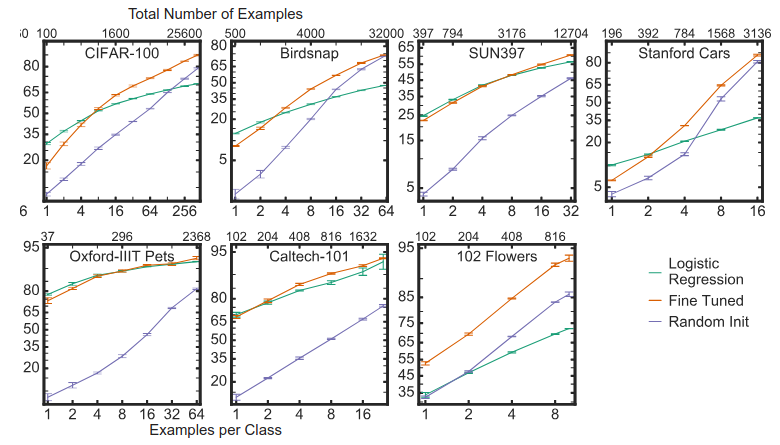
\includegraphics[width=0.8\textwidth]{images/LT3.png}
    \caption{Image from "Do better ImageNet model transfer better"}
    \label{fig:MHA2}
\end{figure}
This image analyzes the behavior of fine-tuning in scenarios where only a small number of
training examples per class are available.
The curves compare logistic regression, fine-tuning, and training from random initialization
as the number of samples increases.

The results show that pretraining on ImageNet provides a significant advantage when data is
scarce, especially for fine-grained recognition tasks.
In the low-data regime, fine-tuning consistently outperforms both logistic regression and
random initialization, highlighting the strong prior induced by pretrained representations.
As the dataset size grows, the performance gap gradually narrows, since models trained from
scratch can eventually learn suitable representations.

\subsection{Fine-Tuning and Faster Convergence}
\begin{figure}[H]
    \centering
    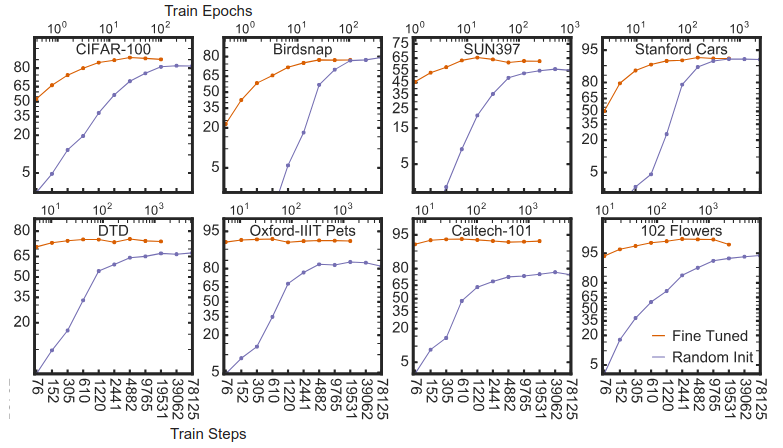
\includegraphics[width=0.8\textwidth]{images/LT4.png}
    \caption{Image from "Do better ImageNet model transfer better"}
    \label{fig:MHA2}
\end{figure}
This image illustrates the effect of fine-tuning on training dynamics by comparing convergence
speed.
Models pretrained on ImageNet are contrasted with models trained from random initialization
as a function of training steps.

The plots show that pretrained networks converge much faster, reaching high accuracy in far
fewer training iterations.
Even when the final accuracy achieved by both approaches is similar, fine-tuning offers a
clear optimization advantage by starting from parameters that are already close to a good
solution.
This faster convergence reduces training time and computational cost, further motivating the
use of transfer learning in practice.

\subsection{Why Has Fine-Tuning Become So Dominant?}
\begin{wrapfigure}{r}{0.2\textwidth}
    \centering
    \vspace{-10pt}
    
\includegraphics[width=\linewidth]{images/LT5.png}
    \label{fig:Scaled Dot Product Attention}
    \vspace{-10pt}
\end{wrapfigure}
Fine-tuning has become the dominant paradigm in modern deep learning due to a combination of
practical and computational advantages.

First, it enables extensive \textbf{reuse}. Modern frameworks and libraries provide access to
large collections of pretrained models whose weights can be easily adapted to new tasks with
minimal additional training. This avoids the massive computational cost required for training
large models from scratch and significantly reduces the time-to-market when deploying machine
learning solutions.

Second, fine-tuning leads to a reduced \textbf{design effort}. Pretrained models are typically
associated with well-tested architectures, including carefully chosen layers, activation
functions, and hyperparameters. These design choices have been validated by extensive research
and benchmarking, allowing practitioners to focus on the specifics of the target problem rather
than on architectural exploration or low-level model tuning.

\subsection{Technical Aspects of Fine-Tuning}
One of the key technical decisions in fine-tuning concerns whether to \textbf{freeze some layers}
of the pretrained network. Earlier layers typically capture generic, low-level features such as
edges, textures, and simple patterns, which are often transferable across different tasks.
For this reason, these layers can be reused and kept fixed during fine-tuning, while higher
layers are adapted to the target task.

Freezing layers provides several advantages:
\begin{compactitemize}
    \item \textbf{Reduced computation}: frozen layers can be set to \texttt{no\_grad}, lowering
    memory usage and eliminating gradient-related FLOPs;
    \item \textbf{Faster convergence}: the optimizer focuses only on adapting task-specific
    layers, requiring fewer parameter updates, which speeds up training;
    \item \textbf{Stability}: freezing early layers helps prevent the degradation of useful
    generic representations learned on the source task;
    \item \textbf{Preserved generalization}: early layers encode low-level, task-agnostic features
    such as edges, textures, and simple visual patterns that generalize well across domains.
    Keeping these layers fixed preserves the inductive bias learned on the source task and acts
    as a form of regularization, reducing the risk of overfitting when the target dataset is
    small and leading to more consistent and reliable performance.
\end{compactitemize}

\begin{figure}[H]
    \centering
    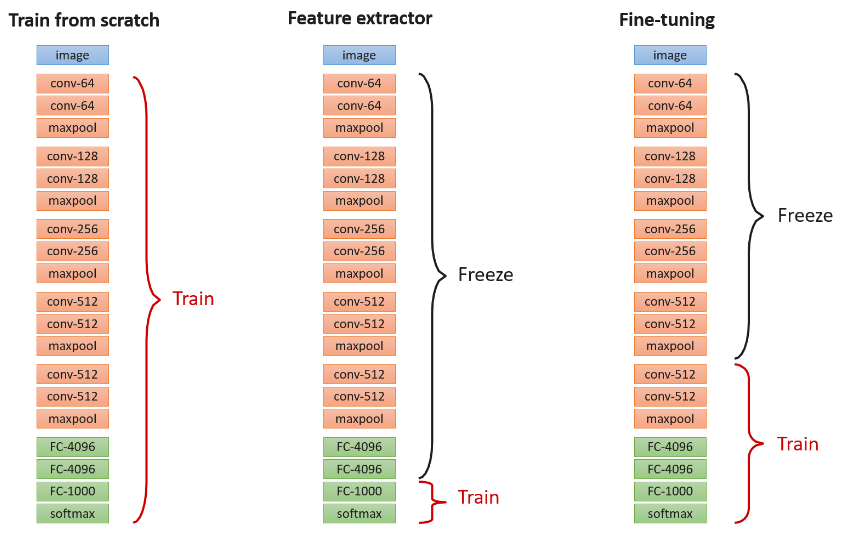
\includegraphics[width=0.8\textwidth]{images/LT6.png}
    \label{fig:MHA2}
\end{figure}


Different fine-tuning strategies can be adopted depending on how many layers are trained:
\begin{compactitemize}
    \item \textbf{Last layer only}: only the classifier is trained. This approach enables very
    fast adaptation with a low risk of overfitting, but offers limited flexibility. It is also
    known as \textbf{linear probing};
    \item \textbf{Last $N$ layers}: strikes a balance between adaptation capacity and overfitting
    risk by allowing partial modification of the pretrained representation;
    \item \textbf{All layers}: the entire network is fine-tuned, providing maximum flexibility at
    the cost of higher computational requirements and an increased risk of overfitting.
\end{compactitemize}

\begin{figure}[H]
    \centering
    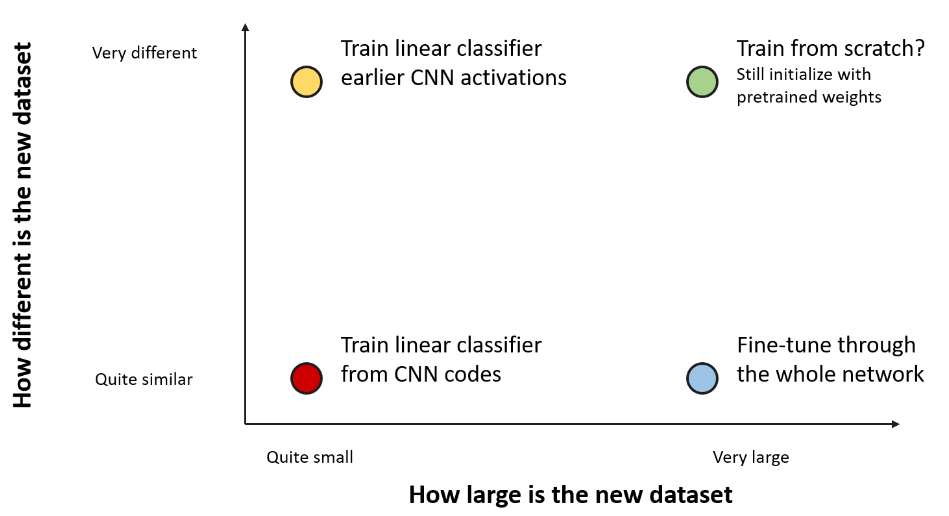
\includegraphics[width=0.7
    \textwidth]{images/LT7.png}
    \label{fig:MHA2}
\end{figure}

\begin{infobox}[Note]
    Note that linear probing is often used in the literature as a quick diagnostic tool to evaluate
the quality and transferability of features produced by a frozen backbone on downstream tasks.
\end{infobox}

\subsection{Learning Rate Strategies during Fine-Tuning}
The choice of the learning rate and its scheduling plays a crucial role in effective fine-tuning,
as pretrained networks are sensitive to large parameter updates that may destroy useful
representations learned on the source task.

A simple approach is to use a \textbf{uniform learning rate}, where the same learning rate is
applied to all trainable layers. This strategy is easy to implement and works reasonably well
in practice, but it can be suboptimal: early layers may be over-updated, damaging generic
features, or under-updated, limiting adaptation.

A more effective strategy is to adopt \textbf{layer-specific learning rates}, assigning larger
learning rates to the last, task-specific layers and smaller ones to earlier layers. This
encourages rapid adaptation of high-level features while preserving low-level, transferable
representations. This technique is also known as the \textbf{Slow Learner} approach.

Finally, \textbf{learning rate warmup schedules} are often used during fine-tuning, especially
when updating all layers. The idea is to gradually increase the learning rate during the initial
training iterations, preventing sudden large updates that could destabilize pretrained weights
and lead to poor convergence. Essentially we wait until the NN is comfortable with the new data.

\subsection{An Alternative: LP-FT}
\begin{wrapfigure}{r}{0.6\textwidth}
    \centering
    \vspace{-10pt}
    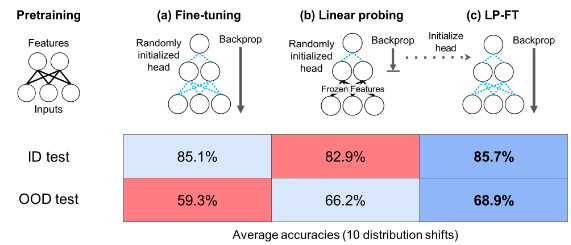
\includegraphics[width=\linewidth]{images/LT8.png}
    \label{fig:Scaled Dot Product Attention}
    \vspace{-10pt}
\end{wrapfigure}
Standard fine-tuning, while effective on in-distribution (ID) data, can sometimes distort
pretrained features, leading to degraded performance when the model is evaluated on
out-of-distribution (OOD) data. This issue becomes particularly relevant under large
distribution shifts, where aggressive parameter updates may harm previously learned
transferable representations.

To address this problem, has been propose proposes the \textbf{LP-FT} strategy
(\textit{Linear Probing + Fine-Tuning}), which combines the strengths of linear probing and
fine-tuning in a two-stage procedure:
\begin{enumerate}
    \item \textbf{Linear probing}: the pretrained backbone is frozen and only a linear
    classification head is trained on the target task. This step adapts the classifier to the
    pretrained feature space without modifying the feature extractor.
    \item \textbf{Fine-tuning}: starting from the adapted classifier, the entire network is
    fine-tuned end-to-end on the target data.
\end{enumerate}

The intuition behind LP-FT is that linear probing provides a well-aligned initialization for the
task-specific head, reducing harmful gradients flowing into the backbone during subsequent
fine-tuning. As a result, the pretrained features are better preserved, leading to improved
generalization.

Another explanation for the effectiveness of this method is that, once linear probing is
completed and the classification head is properly trained, the head guides the subsequent
updates of the backbone during fine-tuning.
As a result, the gradients reaching the backbone are smaller, more stable, and more
task-targeted.

This mechanism helps prevent excessive distortion of pretrained features, allowing the model
to adapt to the target task while preserving the useful representations learned on the source
domain.
Empirical results show that LP-FT achieves higher accuracy than standard fine-tuning both on
ID data and under various OOD shifts, confirming that initializing fine-tuning with a probed
head can mitigate feature distortion and enhance robustness.

\subsection{Batch Normalization in Fine-Tuning}
During fine-tuning, Batch Normalization (BN) layers require special attention.
In some settings, even when the network weights are kept frozen, the \textbf{BatchNorm
statistics} are updated to better match the target domain.
In particular:
\begin{compactitemize}
    \item only the \textbf{running mean} and \textbf{running variance} of the BatchNorm layers are
    updated;
    \item the learnable parameters $\gamma$ (scale) and $\beta$ (shift) can either be kept fixed
    or allowed to update, depending on the fine-tuning strategy.
\end{compactitemize}

Updating only the BN statistics is equivalent to running one training epoch with SGD and
learning rate set to zero: model weights do not change, but normalization statistics gradually
adapt to the target data distribution.

The intuition behind this approach is that it allows the model to \textbf{align feature
normalization to the target domain} without altering the learned representations themselves.
This can significantly reduce distribution mismatch between source and target domains.

For this reason, BN statistics adaptation is widely used in \textbf{domain adaptation} settings,
where the goal is to improve generalization across different data distributions while
minimizing changes to the pretrained model.

\subsection{Limitations of Fine-Tuning}
Some limitations of fini tuning are:
\begin{compactitemize}
    \item \textbf{Architectural rigidity}: Inherits the architecture of the pretrained model, which may not be optimal for the new task (e.g. too many layers -> computational overhead)
    \item \textbf{Dependence on external data/models}: Requires access to pretrained models and their associated datasets, including potential licensing or usage restrictions.
    \item \textbf{Inherited biases}: Any biases present in the source dataset can be transferred and potentially amplified in the target task.
\end{compactitemize}

\begin{figure}[H]
    \centering
    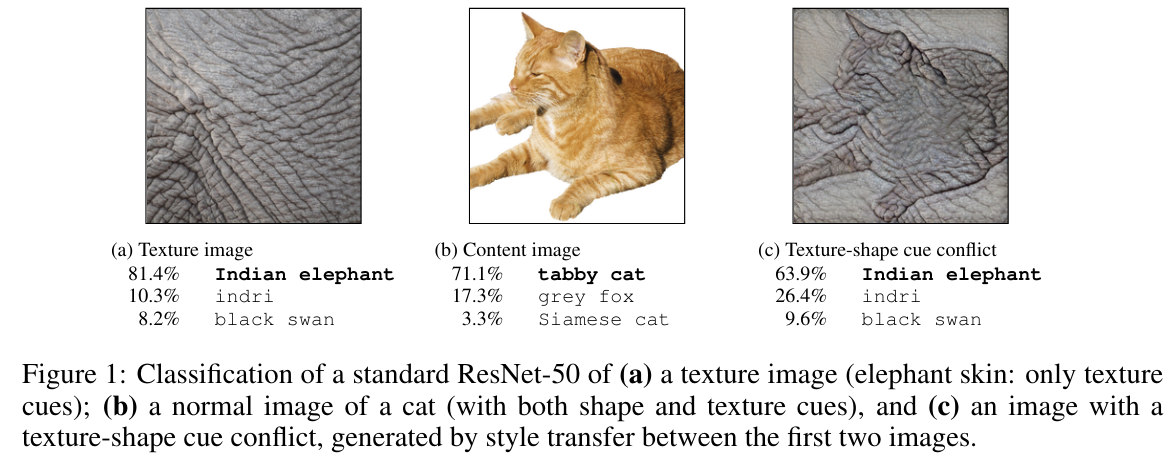
\includegraphics[width=0.9
    \textwidth]{images/LT9.png}
    \label{fig:MHA2}
\end{figure}
\begin{figure}[H]
    \centering
    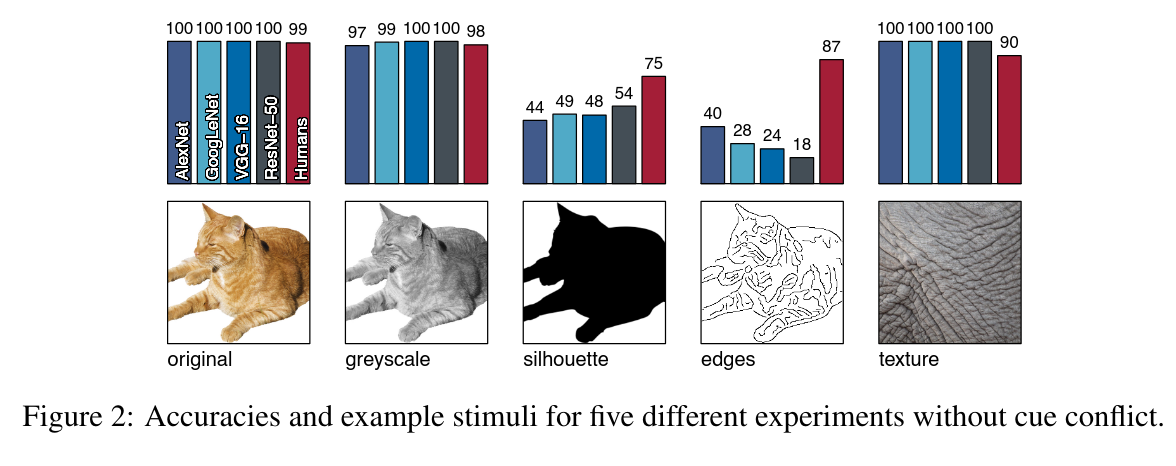
\includegraphics[width=0.9
    \textwidth]{images/LT10.png}
    \label{fig:MHA2}
\end{figure}

The figure shows that a standard ResNet relies predominantly on \textbf{texture cues} rather than
on object shape when performing image classification. In the presence of a texture–shape
conflict, the network tends to predict the class suggested by the texture, revealing a strong
texture bias.

This experiment further confirms that ImageNet-trained ResNet models inherit a
\textbf{bias toward texture-based features}. Even when shape information is preserved or
isolated, classification accuracy remains high only when texture information is available,
highlighting the limited role of global shape in the learned representations.

\subsubsection{Model Storage}
A major limitation of standard fine-tuning is its \textbf{large storage requirement}.
Fine-tuning updates the entire set of model parameters, which implies that a separate copy of
the full model must be stored for each downstream task.

For large models, such as large language models with billions of parameters, this results in a
significant memory and disk footprint per task.
Maintaining multiple fine-tuned versions of the same base model becomes costly and inefficient,
especially when deploying systems at scale.

Additionally, this approach is inflexible in resource-constrained settings, where switching
between tasks may require loading different large model checkpoints, incurring high latency
and memory overhead.

To address these limitations, more recent approaches focus on
\textbf{Parameter-Efficient Fine-Tuning (PEFT)}, such as LoRA, adapters, and prefix-tuning, which
enable task adaptation while drastically reducing storage and memory costs.

\section{Teacher-Student approaches}

\subsection{Deep Ensembles and Impact of Depth}
\begin{wrapfigure}{r}{0.5\textwidth}
    \centering
    \vspace{-10pt}
    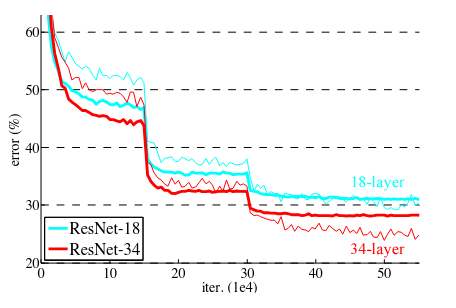
\includegraphics[width=\linewidth]{images/LT11.png}
    \label{fig:Scaled Dot Product Attention}
    \vspace{-10pt}
\end{wrapfigure}
It is well known that increasing the depth of a neural network enables the model to learn more
complex patterns and richer hierarchical representations, often leading to improved
performance compared to smaller models.

Similarly, \textbf{deep ensembles}, where multiple models are trained independently and converge
to different local minima, typically achieve stronger performance and improved robustness with
respect to single models.

These two approaches share important similarities:
\begin{compactitemize}
    \item both rely on \textbf{redundancy of representations} to improve accuracy and robustness;
    \item both generally achieve \textbf{very strong results} across a wide range of tasks.
\end{compactitemize}

Despite their effectiveness, both deeper models and ensemble methods present a major drawback:
they are often \textbf{hard to deploy in production} due to high computational and memory
requirements.
In practical scenarios, especially at test time, it is crucial to minimize computational cost
and memory footprint, as these constraints are typically much more severe during inference than
during training.

\subsection{The Insects Parallelism}

The insects parallelism provides an intuitive analogy for understanding modern large-scale
machine learning systems and their lifecycle.

Many insects have two very different stages. In the \textbf{larval stage}, the organism is
optimized for extracting energy and nutrients from the environment. This stage is slow,
resource-intensive, but extremely effective at growth.  
Similarly, during the \textbf{training stage} in machine learning, large and complex models
— often deep, redundant, and heavily regularized — are used to extract structure and knowledge
from massive datasets. At this stage, efficiency is not the primary concern.

In contrast, the \textbf{adult stage} (the butterfly) is optimized for mobility and survival,
operating efficiently with limited resources.  
This mirrors the \textbf{deployment stage} of machine learning models, where systems must
perform inference in real time, at scale, and under strict computational and memory constraints.

\begin{figure}[H]
    \centering
    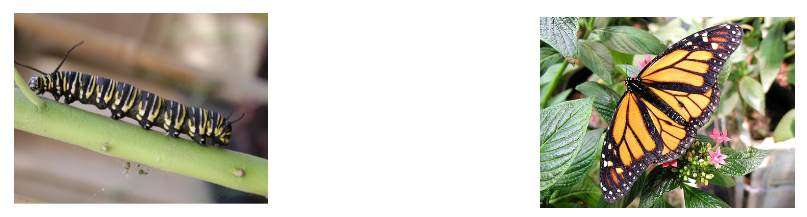
\includegraphics[width=0.9\textwidth]
    {images/LT12.png}
    \label{fig:MHA2}
\end{figure}

The key insight of this perspective is that \textbf{learning and deployment have different
requirements}. A large and complex model is ideal for learning, but not for deployment.
Therefore, the goal is to first train a powerful \emph{larval} model to simplify learning, and
then transfer the acquired knowledge into a smaller and more efficient \emph{butterfly} model
that is suitable for real-world use.

In this view, ensembles or large models are treated as a function mapping inputs to outputs.
Once this function is learned, the internal structure and parameterization of the model become
secondary.  
The central question then becomes: \emph{can we transfer the knowledge stored in this function
into a single, smaller model?}
This question naturally leads to techniques such as \textbf{knowledge distillation}, which aim
to bridge the gap between powerful learners and efficient deployable models.

\subsection{Knowledge Distillation}
\begin{wrapfigure}{r}{0.4\textwidth}
    \centering
    \vspace{-10pt}
    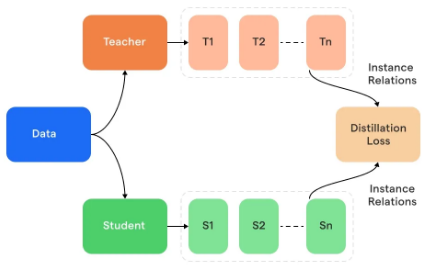
\includegraphics[width=\linewidth]{images/LT13.png}
    \label{fig:Scaled Dot Product Attention}
    \vspace{-10pt}
\end{wrapfigure}
\textbf{Knowledge Distillation (KD)} is a technique designed to transfer knowledge from a large,
complex model (the \textbf{teacher}) to a smaller and more efficient model (the \textbf{student}).
The main idea is to train the student not only using ground-truth labels, but also to mimic the
output distribution produced by the teacher.

\newpage
The teacher model can be:
\begin{compactitemize}
    \item a single, large and cumbersome model (e.g. deeper or wider architecture);
    \item an ensemble of multiple models, whose predictions are averaged to obtain more reliable
    outputs.
\end{compactitemize}

\subsubsection{Softened Probabilities}
\begin{wrapfigure}{r}{0.5\textwidth}
    \centering
    \vspace{-10pt}
    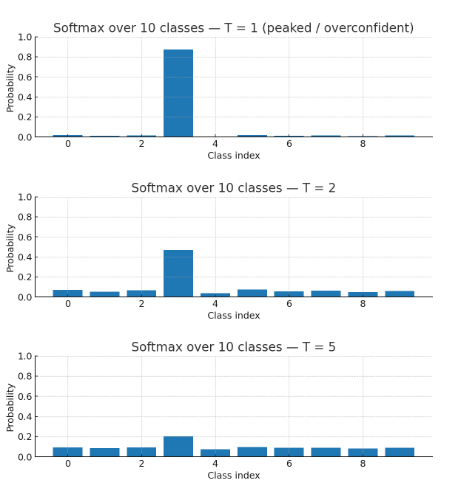
\includegraphics[width=\linewidth]{images/LT14.png}
    \label{fig:Scaled Dot Product Attention}
    \vspace{-10pt}
\end{wrapfigure}
During distillation, the teacher produces logits $z_i$ for each class $i$.
Instead of applying the standard softmax, a \textbf{temperature-scaled softmax} is used:
\[
p_i^{(T)} = \frac{\exp(z_i / T)}{\sum_j \exp(z_j / T)}, \qquad T > 1
\]
A higher temperature $T$ produces a \textbf{softer probability distribution}, characterized by:
\begin{compactitemize}
    \item lower confidence in the top predicted class;
    \item higher probability mass assigned to classes considered similar by the teacher.
\end{compactitemize}
At inference time, the temperature is set back to $T = 1$.

These softened probabilities encode what is often called \textbf{dark knowledge}, i.e. information
about inter-class similarities that is not present in one-hot labels.

\subsubsection{Training Procedure}
The distillation process follows a two-model training loop:
\begin{enumerate}
    \item perform a forward pass with the teacher to compute teacher logits $z_t$;
    \item perform a forward pass with the student to compute student logits $z_s$;
    \item update the student parameters by minimizing a mixed loss function:
\end{enumerate}

\[
\mathcal{L}_{\text{student}} =
\alpha \, \mathcal{L}_{\text{CE}}(y, \sigma(z_s))
+ (1 - \alpha) \, T^2 \, \mathcal{L}_{\text{CE}}\big(\sigma(z_t/T), \sigma(z_s/T)\big)
\]

where:
\begin{compactitemize}
    \item $y$ is the ground-truth one-hot label;
    \item $\sigma(\cdot)$ denotes the softmax function;
    \item $T$ is the distillation temperature;
    \item $\alpha$ balances hard targets and soft targets.
\end{compactitemize}

\subsubsection{Effectiveness of Knowledge Distillation}
Empirically, incorporating soft targets during training typically improves performance compared
to using hard labels alone, often yielding:
\[
\text{KD} \; > \; \text{Student trained from scratch}
\]

Experimental results on CIFAR-100 confirm that distillation consistently improves student
accuracy, even when teacher and student architectures differ. This demonstrates that the
knowledge transferred through softened outputs is not tightly coupled to a specific
architecture, but captures more general and transferable patterns learned by the teacher.

\subsection{Dark Knowledge}
\textbf{Dark knowledge} refers to the information contained in the relative probabilities
assigned by a model to the \textbf{non-argmax classes}, also known as secondary information.
Unlike one-hot labels, which provide supervision only for the correct class, dark knowledge
encodes the similarity structure between classes learned by the teacher model.

For example, given an image of a cat, a teacher model may produce an output distribution such as:
\[
[\text{Cat}: 0.65,\; \text{Dog}: 0.25,\; \text{Fox}: 0.07]
\]
This distribution reveals that the teacher considers dogs more similar to cats than foxes, an
insight that is completely lost when using hard one-hot targets.

These secondary probabilities guide the student to learn \textbf{richer and smoother decision
boundaries} than those induced by standard supervision alone. In particular, each training
example provides constraints on multiple class relationships, rather than enforcing a single,
hard decision.

As a result, soft targets act as a \textbf{powerful regularizer}, discouraging overconfident
predictions and improving generalization. This regularization effect is a key reason why
knowledge distillation often leads to better performance and more robust models.

\subsection{Distillation via Pre-Softmax Activations}
An alternative approach to standard knowledge distillation goes beyond probability matching.
Instead of aligning the softened output probabilities of teacher and student, it directly
matches their \textbf{pre-softmax activations} (logits).

Let $z_t$ and $z_s$ denote the logits produced by the teacher and the student, respectively.
Logit-based distillation minimizes the Mean Squared Error (MSE) between them:
\[
\mathcal{L}_{\text{logit}} = \frac{1}{K} \sum_{i=1}^{K} (z_{t,i} - z_{s,i})^2
\]
where $K$ is the number of classes.

This loss can be combined with the standard cross-entropy loss computed using the true labels,
allowing the student to learn both from ground-truth supervision and from the teacher’s
internal representations.

One key advantage of logit-based distillation is that it avoids potential information loss
introduced by the softmax transformation, which can compress or obscure differences between
classes. By operating directly on logits, the method emphasizes the transfer of secondary
information related to class similarities and relative confidence levels learned by the
teacher, leading to more faithful knowledge transfer.

\subsection{Applications of Knowledge Distillation}
Knowledge distillation is a versatile technique with wide applicability across different stages
of model development and deployment.

A primary application is \textbf{model compression}. By distilling knowledge from a large
teacher into a smaller student, it is possible to significantly reduce memory footprint and
computational cost, enabling deployment on edge devices and mobile platforms.

Closely related is \textbf{latency reduction}. Distilled models are typically faster at
inference time, making them suitable for real-time applications such as speech recognition,
video analytics, and online recommendation systems.

Another common use case is \textbf{ensemble-to-single transfer}. Instead of deploying a large
and expensive ensemble of models, knowledge distillation allows transferring most of the
ensemble’s accuracy into a single compact model, greatly simplifying deployment.

Knowledge distillation is also effective for \textbf{cross-architecture transfer}. For example,
knowledge can be distilled from a CNN to a Transformer, or vice versa, allowing the student to
benefit from the strengths of a different architectural family.

In \textbf{domain adaptation} settings, a teacher trained on one domain can guide a student
operating on a related but different domain, helping reduce distribution mismatch and improve
generalization.

Finally, distillation can act as a form of \textbf{regularization during training}. In
self-distillation, a model is trained to match its own earlier predictions, which encourages
consistency and often leads to improved generalization even without an external teacher.

\subsection{Similarity-Preserving Knowledge Distillation}
\begin{wrapfigure}{r}{0.5\textwidth}
    \centering
    \vspace{-10pt}
    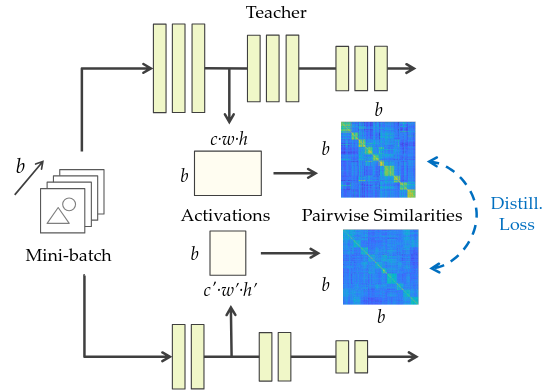
\includegraphics[width=\linewidth]{images/LT15.png}
    \label{fig:Scaled Dot Product Attention}
    \vspace{-10pt}
\end{wrapfigure}
Similarity-Preserving Knowledge Distillation is an extension of standard knowledge distillation
that aims to transfer not only the output predictions of a teacher model, but also the
\textbf{relational structure} of the data learned in its feature space.

The key motivation is that the relationships between samples in the embedding space contain rich
semantic information that goes beyond individual class predictions. Semantically similar inputs
tend to produce similar activation patterns in a well-trained network, and preserving these
relationships can significantly improve knowledge transfer.

In this approach, feature representations are extracted from both the teacher and the student,
and pairwise similarity matrices are computed:
\begin{compactitemize}
    \item $S_T$: similarity matrix between samples in the teacher feature space;
    \item $S_S$: similarity matrix between samples in the student feature space.
\end{compactitemize}

In addition to the standard cross-entropy or distillation loss, the student is trained by
minimizing a similarity-preserving loss of the form:
\[
\mathcal{L}_{\text{SP}} = \lVert S_T - S_S \rVert_F^2
\]
where $\lVert \cdot \rVert_F$ denotes the Frobenius norm.

By aligning the similarity structure of the student with that of the teacher, this method
encourages the student to capture the same geometric organization of the data in the embedding
space. As a result, the student inherits a deeper form of knowledge that reflects how the
teacher organizes and disentangles data, leading to improved generalization and more robust
representations.

\subsection{Paying More Attention to Attention}

Attention Transfer (AT) is a knowledge distillation technique that focuses on transferring the
\textbf{spatial attention maps} from a teacher to a student model. Instead of matching full
feature maps—which may differ in dimensionality or structure—AT encourages the student to
replicate the teacher’s attention, i.e., the regions of the input that the teacher considers most
informative.
\begin{wrapfigure}{r}{0.3\textwidth}
    \centering
    \vspace{-10pt}
    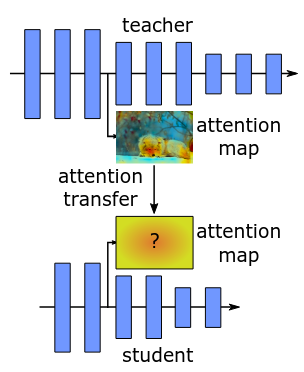
\includegraphics[width=\linewidth]{images/LT16.png}
    \label{fig:Scaled Dot Product Attention}
    \vspace{-10pt}
\end{wrapfigure}
The intuition is straightforward: attention maps highlight \textbf{where} the model focuses
during prediction. By imitating the teacher’s attention patterns, the student learns not only
\emph{what} to predict, but also \emph{where to look}. This improves knowledge transfer, even
when teacher and student differ significantly in architecture or depth.

To compute attention maps, consider feature maps $F \in \mathbb{R}^{C \times H \times W}$, where
$C$ is the number of channels. The spatial attention map is obtained by aggregating across
channels:
\[
A = \frac{1}{C} \sum_{c=1}^{C} |F_c|^p,
\qquad p \in \{1, 2\}
\]

Each attention map is then normalized to unit norm:
\[
\hat{A} = \frac{A}{\lVert A \rVert_2}
\]

Attention transfer is performed by minimizing the squared distance between the normalized
attention maps of teacher and student:
\[
\mathcal{L}_{AT} = \lVert \hat{A}_T - \hat{A}_S \rVert_2^2
\]

This loss is typically combined with standard cross-entropy or knowledge-distillation losses.
By guiding the student to mimic the teacher’s attention behavior, AT helps the student learn
more effective and interpretable feature representations, improving generalization and
transferability.

\begin{figure}[H]
    \centering
    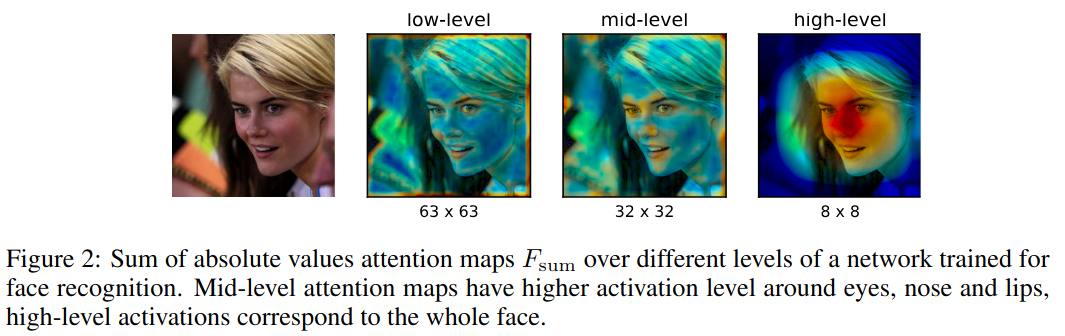
\includegraphics[width=0.9
    \textwidth]{images/LT17.png}
    \label{fig:MHA2}
\end{figure}

\subsection{FitNets: Hints for Thin Deep Networks}
FitNets extend standard knowledge distillation by transferring \textbf{intermediate feature
representations} from the teacher to the student, rather than relying only on the final output
logits. This is particularly useful when the student network is very deep but thin, a setting
in which training from scratch can be difficult and unstable.
\begin{wrapfigure}{r}{0.6\textwidth}
    \centering
    \vspace{-10pt}
    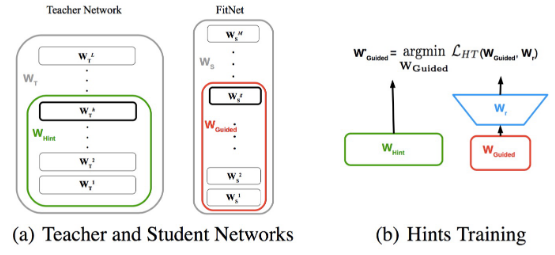
\includegraphics[width=\linewidth]{images/LT18.png}
    \label{fig:Scaled Dot Product Attention}
    \vspace{-10pt}
\end{wrapfigure}
The key motivation behind FitNets is that providing intermediate \emph{hints} from the teacher
helps guide the optimization of the student, easing the learning of meaningful representations
layer by layer instead of only through end-task supervision.

The method works as follows:
\begin{compactitemize}
    \item a \textbf{hint layer} is selected in the teacher network, typically a deep intermediate
    layer containing rich semantic information;
    \item a corresponding \textbf{guided layer} is selected in the student network, usually at a
    similar depth;
    \item if the feature dimensions do not match, a small \textbf{regressor} (e.g., a $1\times1$
    convolution or an MLP) is applied to map the student features into the teacher’s feature
    space.
\end{compactitemize}

In addition to the standard knowledge distillation or cross-entropy loss on the outputs,
FitNets minimize a hint-based loss defined as:
\[
\mathcal{L}_{\text{hint}} = \lVert r(f_S) - f_T \rVert_2^2
\]
where $f_S$ and $f_T$ denote the student and teacher feature representations at the guided and
hint layers, and $r(\cdot)$ is the regressor.

There are no strict rules for choosing hint and guided layers; the selection depends on the
architecture. In practice, choosing layers at comparable depths is a common and effective
strategy.

A key advantage of FitNets is their flexibility. They are not limited to teacher–student pairs
with similar depth or width and can be applied when:
\begin{compactitemize}
    \item the student is deeper but thinner than the teacher;
    \item the student is shallower or has a different architecture;
    \item the teacher and student have different hidden layer sizes.
\end{compactitemize}

This flexibility makes FitNets a powerful distillation technique for training compact yet deep
models while preserving much of the representational power of larger networks.

\subsection{Self-Knowledge Distillation}
\textbf{Self-Knowledge Distillation (Self-KD)} applies the distillation paradigm to two networks
that share the \textbf{same architecture}. In this case, the difference between teacher and
student does not lie in model capacity, but in the \textbf{information content of the inputs}
they receive.

In a typical setup:
\begin{compactitemize}
    \item the \textbf{teacher} is trained using richer or more informative inputs (e.g., multiple
    modalities, full-resolution data, or clean signals);
    \item the \textbf{student} is trained using degraded, partial, or noisier versions of the
    same inputs.
\end{compactitemize}

During training, a distillation loss encourages the student to match the teacher’s intermediate
feature representations or final output predictions, despite having access to less information.

The main benefit of Self-KD is that it shifts the learning challenge from \textbf{model capacity}
to \textbf{input efficiency}. Rather than relying on a larger or more complex architecture, the
student learns to extract more informative and discriminative patterns from limited data.

Interestingly, in some scenarios the student can even \textbf{surpass the teacher}, as the
distillation process acts as a strong regularizer and promotes more robust representations.

Self-KD is particularly useful in real-world settings involving \textbf{missing modalities},
partial observations, or low-quality inputs, where models must operate effectively under
information constraints.

\subsection{Applications to Video Recognition}
Self-Knowledge Distillation can be effectively applied to \textbf{video recognition} tasks such
as object tracking and video-based person re-identification, where temporal information plays a
crucial role.

In this setting, both the teacher and the student share the same network architecture (e.g.,
ResNet-50), but differ in the number of input frames they process. The \textbf{teacher} is trained
using a larger and more informative set of video frames, while the \textbf{student} is trained
using fewer frames, thus receiving limited temporal context.

The distillation loss encourages the student to match the teacher’s feature representations or
final predictions, forcing it to exploit richer temporal and spatial cues from reduced visual
evidence. Through this process, the student learns to compactly encode motion and appearance
information that would otherwise require longer sequences.

\begin{wrapfigure}{r}{0.7\textwidth}
    \centering
    \vspace{-10pt}
    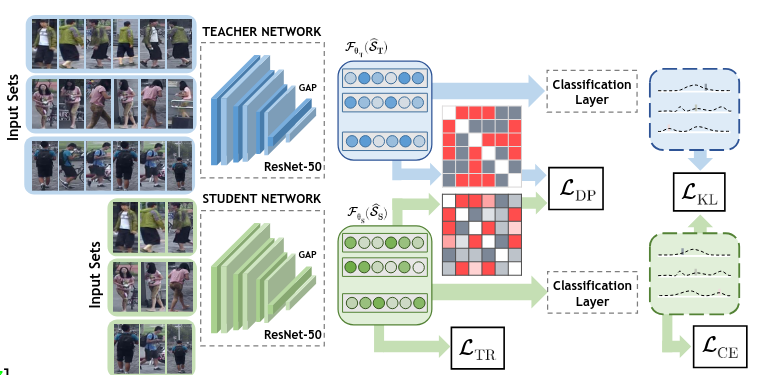
\includegraphics[width=\linewidth]{images/LT19.png}
    \label{fig:Scaled Dot Product Attention}
    \vspace{-10pt}
\end{wrapfigure}

This approach allows the deployment of video recognition models with lower computational cost
and latency, while retaining competitive performance. As a result, Self-KD is particularly
well-suited for real-time video applications where memory, bandwidth, or frame availability are
limited.
